\section{通用实验设定}
\paragraph{\textbf{目标模型。}} 除非特别说明，我们从通用的指令微调 LLM（例如 Llama-3.1-8B-Instruct~\citep{dubey2024llama}）出发。该模型经过常规预训练和监督微调，但没有针对长链式思维链进行优化。\vspace{-5pt}

\paragraph{\textbf{数据来源。}} 我们从 OpenThoughts-3~\citep{guha2025openthoughts} 随机采样 20K--35K 高质量 Long CoT 查询作为主要训练语料。该数据集提供多步推理轨迹，每个样本平均超过 20 步，涵盖多种数学与逻辑问题类型。\vspace{-5pt}

\paragraph{\textbf{评测基准。}} 我们在 6 个需要多步逻辑推理的挑战性数学基准上评估模型：
\begin{itemize}[leftmargin=16pt, itemsep=0pt, topsep=0pt]
  \item \textbf{GSM8K~\citep{cobbe2021training}:} 小学数学题，强调多步计算；
  \item \textbf{MATH-500~\citep{hendrycks2021measuring}:} 面向高中/大学初级难度，覆盖主流数学分支；
  \item \textbf{AMC 2023~\citep{amc2023}:} 高中竞赛题，含代数、几何、组合内容；
  \item \textbf{AIME 2024~\citep{aime2024}:} AIME 级难度，答案为整数；
  \item \textbf{AIME 2025~\citep{aime2025}}；
  \item \textbf{OlymBench~\citep{he2024olympiadbench}:} 全面的奥赛级推理基准。
\end{itemize}
若无特殊说明，“Overall” 指上述基准的平均准确率。\vspace{-5pt}

\paragraph{\textbf{推理与度量。}}
评测时，我们沿用强化学习阶段的采样温度 $=0.6$，以减少 SFT 与 RL 的分布差距。对于 GSM8K、MATH-500 与 OlymBench，我们汇报 Avg@1 准确率；对于 AMC 2023 与 AIME 2024/2025 这类较小测试集，我们报告 Avg@16。模型被要求用 $\setminus$boxed\{$\cdot$\} 输出最终答案，方便解析；解析后再与参考答案对齐，使用标准工具（例如 \texttt{math-verify}）。除非另外说明，其余训练设定保持一致。



\section{冷启动实验的详细设置}
\label{append:preliminary-data}
本附录详细说明 Long CoT 冷启动预研的实验配置。我们比较 3 条数据构建流程。所有流程中，模型均用学习率 $2\mathrm{e}{-5}$、全局 batch size 128 训练 1 个 epoch，最大序列长度设为 \{16K, 32K\} 中表现更好的一个。骨干模型涵盖 Qwen2.5~\citep{yang2024qwen25} 与 Llama3.1~\citep{dubey2024llama}，并在多个规模上冷启动 Long CoT。\vspace{-5pt}

\begin{figure*}[t]
    \centering
    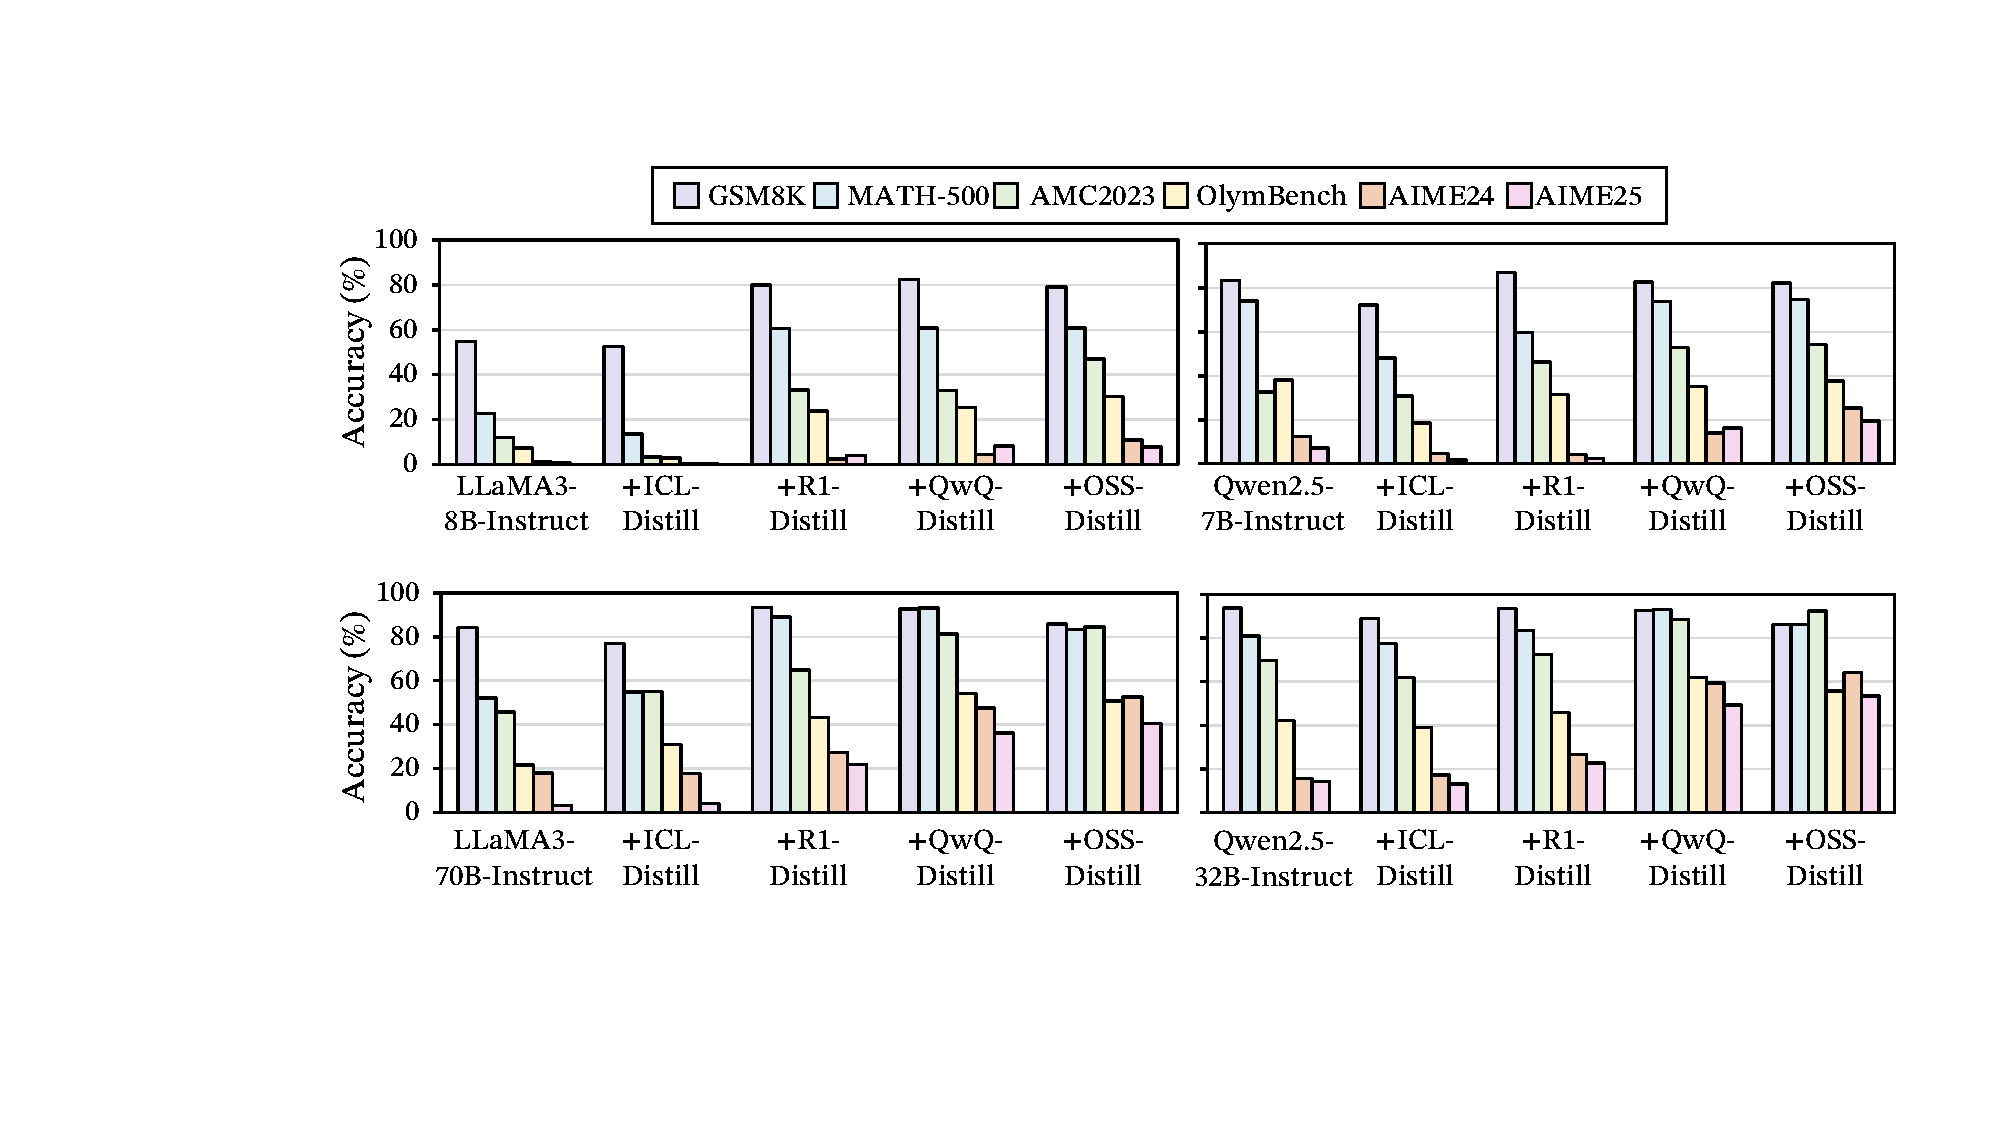
\includegraphics[width=\textwidth]{figures/comparison-full.pdf}
    \caption{弱指令 LLM+ICL 与人类标注轨迹在获取 Long CoT 结构上的完整失败案例，对比成功的强推理模型蒸馏。}
    \label{fig:comparison-full}
\end{figure*}
\paragraph{\textbf{设定 1：来自强推理 LLM 的蒸馏。}}
我们使用大型推理模型生成高质量的合成数据，具体包括 DeepSeek-R1-671B-0528~\citep{guo2025deepseek}、QwQ-32B~\citep{qwq2024} 以及 OpenAI-OSS-120B~\citep{gptoss}。\vspace{-5pt}

\paragraph{\textbf{设定 2：来自弱指令 LLM 的蒸馏（ICL-Distill）。}}
为模拟指令模型通过 ICL 进行表层模仿，我们选用标准指令模型（如 Qwen2.5-32B-Instruct），它并未针对深度推理优化。我们随机从教师的 R1 长链轨迹中选取 1-shot 示范放入提示词，然后让指令模型在与设定 1 相同的问题上生成解答。\vspace{-5pt}

\paragraph{\textbf{设定 3：人类标注轨迹微调。}}
我们使用 50 条 R1 轨迹与 50 条人类逐步解答进行监督微调，对比其效果。数据来源与 \citet{du2025the} 相同。


\section{Long CoT 中的推理键}
本节提供分析 Long CoT 推理键所需的实验细节。

\subsection{推理键的数学定义与分析}
\label{append:math}
\subsubsection{推理行为定义}
给定输入 \(x\)，模型输出含中间推理和最终答案的文本 \(y\)。我们按标准分隔符（换行、列表符号等）把 \(y\) 切分为 \(T\) 个步骤（“steps”）~\citep{golovneva2023roscoe,chen2024unlocking}，得到 Long CoT 轨迹
\begin{equation}
\tau \coloneqq (u_1,\ldots,u_T),
\end{equation}
其中 \(u_t\) 为第 $t$ 个文本步骤。

为分析几何性质，我们把每个步骤 \(u_t\) 映射为向量 \(h_t \in \mathbb{R}^d\)。具体做法：用固定的参考编码器，对每个 token 取固定层（例如倒数第二层）隐状态，然后求平均得到步骤嵌入 \(h_t\)，从而获得序列 \((h_1,\ldots,h_T)\)。

\paragraph{行为空间与带标签的转移。}
我们把 Long CoT 看作步骤之间的转移序列。对 \(t \in \{1,\ldots,T-1\}\)，定义有向转移
\begin{equation}
e_t \coloneqq (u_t \rightarrow u_{t+1}).
\end{equation}
行为标签集合记为
\begin{equation}
\mathcal{B} \coloneqq \{\mathcal{N},\mathcal{D},\mathcal{R},\mathcal{E}\},
\end{equation}
其中 \(\mathcal{N}\) 表示常规操作，\(\mathcal{D}\) 为深层推理，\(\mathcal{R}\) 为自我反思，\(\mathcal{E}\) 为自我探索。自动分类器（见附录 C.1）会为每条连续边 $(h_{t-1}, h_t)$ 打标签，得到序列 $(e_t,b_t)_{t=1}^{T-1}$。

我们据此建立一个“行为图”框架，把分子式“键”对应到可估计、可比较、可迁移的行为边分布。

\paragraph{定义 1（深层推理：\(\mathcal{D}\)）。}
若步骤 \(u_{t+1}\) 的主要意图是通过非平凡推理扩展链条（如多步因果、演绎、类比等），则 \(e_t\) 被标为 \(\mathcal{D}\)。该步骤通常会引入新的潜在假设、中间变量，或是超出简单计算/复述的推理。

\paragraph{定义 2（自我反思：\(\mathcal{R}\)）。}
若 \(u_{t+1}\) 明确评论、审视或调节模型自身的推理过程，如表达不确定性、调整策略、纠错或回溯早期步骤，则标记为 \(\mathcal{R}\)。

\paragraph{定义 3（自我探索：\(\mathcal{E}\)）。}
若 \(u_{t+1}\) 有意分支到新的假设或方案，保持多条路径并行，而非立即收敛，则标为 \(\mathcal{E}\)。

\paragraph{备注（常规操作 \(\mathcal{N}\)）。}
不满足上述条件的转移都记为 \(\mathcal{N}\)，例如直接算术、简单逻辑、格式化输出等。

\paragraph{说明。} 需要注意，连接逻辑节点的边不仅把步骤 $s_t$ 连接到 $s_{t+1}$，还会指向与之相关的早前节点。

\subsubsection{注意力能量的定义}
我们直接从注意力模式入手。对 Transformer 的某一层/头，令 $q_i,k_j$ 分别表示第 $i$、$j$ 个 token 的查询与键。注意力权重
\begin{equation}
    s_{ij} = \frac{q_i^\top k_j}{\sqrt{d_k}}, \quad
    \alpha_{ij} = \frac{\exp (\frac{q_i^\top k_j}{\sqrt{d_k}})}{\sum_{\ell}\exp (\frac{q_i^\top k_\ell}{\sqrt{d_k}})}.
\end{equation}
沿用 Gibbs–Boltzmann 参数化，我们定义“注意力能量”
\begin{equation}
E_{ij} \triangleq -s_{ij} = -\frac{q_i^\top k_j}{\sqrt{d_k}},
\label{eq:attn-energy-def}
\end{equation}
代回即得
\begin{equation}
\alpha_{ij} = \frac{\exp(-E_{ij})}{\sum_{\ell}\exp(-E_{i\ell})},
\end{equation}
这是温度为 1 的玻尔兹曼分布。因而能量越低，对应的注意力越高。

为将其与 Long CoT 行为联系起来，我们使用附录 C.3 的标注流程，把每条转移分类为 Deep/Reflection/Exploration（另有 \(\mathcal{N}\) 作为局部基线）。对每条带标签的边 $b$，我们聚合源、目标步骤之间的 token 级注意力，并用式~\eqref{eq:attn-energy-def} 转成能量值，得到三个随机变量 $E_{\mathcal{D}},E_{\mathcal{R}},E_{\mathcal{E}}$。

\subsubsection{推理键能量的有序性}
为分析不同键的能量排序，我们考虑带 RoPE~\citep{su2024roformer} 的注意力。令
\begin{equation}
q_i = R(i)u_i, \quad k_j = R(j)v_j,
\end{equation}
其中 $R(t)$ 是正交旋转。则
\begin{equation}
s_{ij} = \frac{u_i^\top R(i-j)v_j}{\sqrt{d_k}},
\end{equation}
仅与相对位置有关。

\paragraph{键的随机变量与期望}
设 $d_D=1$（相邻），选择 $1<d_R<d_E$。定义
\begin{equation}
\mathcal{E}_{\mathcal{D}}(i)=E_{i,i-1},\quad 
\mathcal{E}_{\mathcal{R}}(i)=E_{i,i-d_R},\quad
\mathcal{E}_{\mathcal{E}}(i)=E_{i,i-d_E}.
\end{equation}
其均值分别记为
\begin{equation}
\bar E_{\mathcal{D}}=\mathbb{E}(\mathcal{E}_{\mathcal{D}}(i)),\quad
\bar E_{\mathcal{R}}=\mathbb{E}(\mathcal{E}_{\mathcal{R}}(i)),\quad
\bar E_{\mathcal{E}}=\mathbb{E}(\mathcal{E}_{\mathcal{E}}(i)).
\end{equation}
目标是证明 $\bar E_{\mathcal{D}}<\bar E_{\mathcal{R}}<\bar E_{\mathcal{E}}$。

\paragraph{假设}
\textbf{A1（各向同性、随距离衰减的互协方差）。}
存在随距离单调递减的 $\rho(d)\ge0$，使得
\begin{equation}
\mathbb{E}[u_i v_j^\top]=\rho(d)I,
\end{equation}
其中 $d=|i-j|$。

\textbf{A2（旋转的正平均对齐）。}
设
\begin{equation}
\mu(d):=\frac{1}{\sqrt{d_k}}\operatorname{tr}(R(d)).
\end{equation}
假设 \(\mu(d)\) 随 $d$ 非增，并对 $d\in\{1,d_R,d_E\}$ 满足 $\mu(d)\ge\underline{\mu}>0$。

\paragraph{定理 1（RoPE 下的期望排序）。}
在 A1--A2 且 $1<d_R<d_E$ 时，有
\begin{equation}
\bar E_{\mathcal{D}} < \bar E_{\mathcal{R}} < \bar E_{\mathcal{E}}.
\end{equation}

\paragraph{证明。}
计算距离为 $d$ 的期望得分：
\begin{align}
\mathbb{E}[s_{i,i-d}] &= \frac{1}{\sqrt{d_k}}\operatorname{tr}(R(d)\,\mathbb{E}[v_{i-d}u_i^\top]) \\
&= \rho(d)\cdot \frac{1}{\sqrt{d_k}}\operatorname{tr}(R(d)) = \rho(d)\mu(d).
\end{align}
因 A1 得 $\rho(1)>\rho(d_R)>\rho(d_E)$，A2 得 $\mu(1)\ge\mu(d_R)\ge\mu(d_E)\ge\underline{\mu}>0$，于是
\begin{equation}
\mathbb{E}[s_{i,i-1}]>\mathbb{E}[s_{i,i-d_R}]>\mathbb{E}[s_{i,i-d_E}],
\end{equation}
两侧取负即可得到能量排序。

\paragraph{键能差的下界。}
令 $\widehat{s}(d)$ 为 $N$ 次独立采样的平均得分，$\widehat{E}(d)=-\widehat{s}(d)$。假设：

\textbf{A3（次高斯 logits）。}
对每个距离 $d\in\{1,d_R,d_E\}$，居中的得分是 $\sigma^2$-次高斯的，则对任意 $\epsilon>0$ 有
\begin{equation}
\Pr(|\widehat{s}(d)-\mathbb{E}[s(d)]|>\epsilon)\le 2\exp\big(-\frac{N\epsilon^2}{2\sigma^2}\big).
\end{equation}
对三个距离作并集界即可得，当
\begin{equation}
\epsilon=\sigma\sqrt{\frac{2\log(6/\delta)}{N}}
\end{equation}
时，三者同时集中，以至少 $1-\delta$ 的概率成立。
若
\begin{equation}
\mathbb{E}[s(1)]-\mathbb{E}[s(d_R)] > 2\epsilon,\qquad
\mathbb{E}[s(d_R)]-\mathbb{E}[s(d_E)] > 2\epsilon,
\end{equation}
则以至少 $1-\delta$ 的概率，$\widehat{E}_{\mathcal{D}} < \widehat{E}_{\mathcal{R}} < \widehat{E}_{\mathcal{E}}$。

\paragraph{引理（有限样本下的高概率排序）。}
若均值间隙 $\Delta_{DR}>0$、$\Delta_{RE}>0$，则对任意 $0<\epsilon<\min(\Delta_{DR},\Delta_{RE})/2$，当
\begin{equation}
N \ge \frac{2\sigma^2}{\epsilon^2}\log \frac{4}{\delta},
\end{equation}
就有
\begin{equation}
\Pr(\hat{E}_D < \hat{E}_R < \hat{E}_E) \ge 1-\delta.
\end{equation}


\subsubsection{低能量边主导路径聚合}
\paragraph{步骤级依赖图。}
将模型生成的思维链划分为节点集合 \(V\)，配以有向边集合 \(B\)。若步骤 $v$ 对前一步 $u$ 的注意力均值超过阈值，则添加边 $b=(u\to v)$。

\paragraph{边级能量。}
给定 token 级能量 $E_{ij}$，对边 $b=(u\to v)$ 定义跨步骤的 token 对集合
\begin{equation}
\mathcal{C}(u\to v)=\{(i,j): i\in \text{tokens}(u), j\in \text{tokens}(v)\}.
\end{equation}
边能量为该集合上的平均：
\begin{equation}
E_b = \frac{1}{|\mathcal{C}(u\to v)|}\sum_{(i,j)\in \mathcal{C}(u\to v)} E_{ij}.
\end{equation}

\paragraph{推理路径与路径能量。}
从源 $s$ 到目标 $t$ 的路径 $p=(b_1,\ldots,b_L)$，其能量为
\begin{equation}
\mathcal{E}(p)=\sum_{\ell=1}^{L} E_{b_\ell}.
\end{equation}

\paragraph{所有路径的 soft-min（有效能量）。}
记 $\mathcal{P}(s\to t)$ 为所有路径集合，定义
\begin{equation}
\mathcal{E}^\star(s\to t) = -\log \sum_{p\in\mathcal{P}(s\to t)} \exp(-\mathcal{E}(p)),
\end{equation}
对应以能量为权的 log-sum-exp。低能量路径贡献更大。

\paragraph{低能量边定义有效约束。}
设两条路径 $p,p'$ 长度相同，只在位置 $\ell^*$ 不同。若 $E_{b_{\ell^*}} \le E_{b'_{\ell^*}}-\delta$，则
\begin{equation}
\frac{\exp(-\mathcal{E}(p))}{\exp(-\mathcal{E}(p'))} = \exp(\mathcal{E}(p')-\mathcal{E}(p)) \ge \exp(\delta).
\end{equation}
这表明，当所有其他边一致时，用更低能量的边替换，会至少以 $\exp(\delta)$ 的倍数加强该路径的影响力。

\paragraph{分析。}
命题~\ref{prop:low-energy-constraints} 说明，低能量边会持续偏好某些多步依赖，从而在无需化学类比的情况下稳定长链结构。若深层推理边的能量普遍较低，则依赖它们的多跳路径会主导聚合。

\subsubsection{Long CoT 正在寻找更稳定的推理结构}
总体而言，化学反应倾向于形成更低能、更稳定的化合物。类似地，我们假设 Long CoT 学习在寻找低注意力能量的稳定配置。我们在温和的遍历性与有界能量假设下形式化这一直觉。

\paragraph{步骤 1：平稳行为频率。}
假设行为序列 \((s_t)\) 形成不可约、非周期、齐次的马尔可夫链，转移矩阵为 $P$，平稳分布 $\pi$ 满足 $P^\top \pi=\pi$。由遍历定理可知：
\begin{equation}
\frac{1}{T-1}\sum_{t=1}^{T-1}\mathbf{1}[s_t=b] \xrightarrow[T\to\infty]{a.s.} \pi_b, \quad \forall b\in\mathcal{B}.
\end{equation}
\vspace{-5pt}
\paragraph{步骤 2：时间平均能量的分解。}
令 $E_t$ 为第 $t$ 条边的注意力能量，则
\begin{equation}
\widehat{E}_T = \sum_{b\in\mathcal{B}} \Big( \frac{1}{T-1}\sum_{t=1}^{T-1}\mathbf{1}[s_t=b] \Big) \cdot \Big( \frac{\sum_{t=1}^{T-1} E_t\, \mathbf{1}[s_t=b]}{\sum_{t=1}^{T-1}\mathbf{1}[s_t=b]} \Big).
\end{equation}
即全局平均等于按行为频率加权的条件平均。\vspace{-5pt}

\paragraph{步骤 3：条件能量平均的收敛。}
若 $\mathbb{E}[|E_t|]<\infty$ 且在给定 $s_t$ 的条件下 $E_t$ 仅依赖当前行为，则由大数定律有
\begin{equation}
\frac{1}{N_b(T)}\sum_{t:s_t=b} E_t \to \mu_b = \mathbb{E}[E_t\mid s_t=b].
\end{equation}
结合步骤 1 可得
\begin{equation}
\widehat{E}_T \xrightarrow[T\to\infty]{a.s.} \sum_{b\in\mathcal{B}} \pi_b \mu_b.
\end{equation}
\vspace{-5pt}
\paragraph{步骤 4：Gibbs 注意力带来的指数偏好。}
考虑第 $t+1$ 步的查询 token $i$，其候选集合 $\mathcal{S}_t$ 的采样分布为
\begin{equation}
\Pr(\mathcal{S}_t=s_j \mid i) = \frac{\exp(-E_{ij})}{\sum_{s_\ell\in\mathcal{S}_t}\exp(-E_{i\ell})}.
\end{equation}
若对任意行为 $b$，注意力能量落在 $[\mu_b-\Delta, \mu_b+\Delta]$，则对 $b,c$ 有
\begin{equation}
\frac{\Pr(\mathcal{S}_t \in b \mid i)}{\Pr(\mathcal{S}_t \in c \mid i)} \ge \exp((\mu_c-\mu_b)-2\Delta).
\end{equation}
因此，低能量行为在路由中具备指数优势。若深层推理/反思的平均能量与探索存在间隔 $\gamma>0$，且 $2\Delta<\gamma$，那么这些低能转移就会以优势系数 $\exp(\gamma-2\Delta)$ 主导。

综上，Transformer 的注意力机制天然偏好稳定、低能的 Long CoT 结构。


\subsection{Long CoT 中稳定的键分布}
\label{append:stable-bond}
\paragraph{\textbf{推理链生成。}}
为分析跨领域的结构属性，我们使用 OpenThoughts-3~\citep{guha2025openthoughts}（涵盖数学、代码、科学推理），在 DeepSeek-R1-671B、OpenAI-o1、QwQ-32B 上生成 Long CoT 轨迹。生成限制最长 \{16,384, 32,768\} token，温度 $T\in[0,1]$，top-$p=0.95$，使用标准重复惩罚，无额外约束。\vspace{-5pt}


\paragraph{\textbf{键类型标注}}
\label{append:annotation}
沿用 \citet{golovneva2023roscoe,chen2024unlocking} 的做法，我们用换行等分隔词把轨迹切分成步骤，再用 Qwen2.5-32B-Instruct 标注连续步骤之间的边类型。对 200 个样本进行人工验证，宏平均 F1 超过 0.85，验证了自动标注的可靠性。

\begin{PromptBox}{键类型标注提示}
你是一名专家标注员。请把“当前步骤”归入以下行为类别之一：
\begin{itemize}[leftmargin=16pt, itemsep=0pt, topsep=0pt]
    \item 常规操作：直接运算、事实回忆、简单逻辑，未引入新逻辑节点；
    \item 深层推理：多步推理、引入新变量或隐藏假设；
    \item 自我反思：评论或检视自身推理，如不确定、纠错、回顾；
    \item 自我探索：提出新可能、分支或并行路径。
\end{itemize}

决策规则：
\begin{itemize}[leftmargin=16pt, itemsep=0pt, topsep=0pt]
    \item[(1)] 若存在重叠，按意图选择最具体类别：关于推理本身 → 反思；分支/猜测 → 探索；扩展链条 → 深层推理；否则为常规操作。
    \item[(2)] 不根据正确性打标签，只看行为风格。
    \item[(3)] 忽略表面复杂度，长算式若属直接计算仍属常规操作。
    \item[(4)] 若混合，以主导意图为准；若难区分，优先级为：反思 > 探索 > 深层推理 > 常规操作。
\end{itemize}

输出格式（严格）：

\#\#\# \textbf{Behavior:} \{normal operation $|$ deep reasoning $|$ self-reflection $|$ exploration\}
\\

PREVIOUS STEP:

\{\}
\\
CURRENT STEP:

\{\}
\end{PromptBox}


\paragraph{\textbf{转移分布分析}}
\label{app:stable-bond-stability}
为构建图~\ref{fig:transfer}，我们在每个模型-任务组合上随机抽取 $N\in\{0.5k,1k,2k,5k,10k,20k\}$ 的样本，统计相邻行为的转移频率，归一化成转移图。通过对不同模型、不同样本规模的图做皮尔逊相关，我们发现当 $N>2k$ 时相关超过 0.9，进一步增加样本则达到 0.95 以上。

\subsection{Long CoT 中的“逻辑折叠”结构}
\label{app:folding}
为分析推理键的分布与几何特征，我们把所有步骤嵌入统一语义空间，并定义相关度量。

\subsubsection{几何嵌入与可视化}
我们使用 Qwen3-8B~\citep{yang2025qwen3} 对每个步骤取倒数第二层隐状态平均，得到 $\{h_1,\dots,h_T\}$。图~\ref{fig:validation} 通过 t-SNE（余弦距离、5,000 次迭代、early exaggeration=12.0）可视化关键簇，并只展示与目标行为相关的部分。我们定义“逻辑簇” $c(h_t)$：若新点与已有簇距离低于阈值 $\alpha$，则归入该簇。阈值取轨迹中点间距离范围的 $2\%$：
\begin{equation}
\alpha = 0.02 \times (h_{\max}-h_{\min}).
\end{equation}

\subsubsection{折叠的几何指标}
\label{app:folding-metrics}
在向量空间中定义欧氏距离。

\paragraph{自我反思：局部移动与回连。}
度量 $d_t = \lVert h_{t+1}-h_t \rVert_2$ 作为局部移动；回连距离 $r_t = \min_{s<t} \lVert h_{t+1}-h_s \rVert_2$。若 $r_t<\alpha$，则判定为“折返”，81.72\% 的反思满足该条件。\vspace{-5pt}

\paragraph{深层推理：路径长度与簇级距离。}
深层推理通常在局部簇内进行复杂推导。我们测量轨迹长度与簇图距离
\begin{equation}
  g_t = \mathrm{dist}_{\mathcal{G}} (c(h_t), c(h_{t+1})),
\end{equation}
其中 $\mathcal{G}$ 的节点为簇，若两簇距离小于 $\alpha$ 则连边。72.56\% 的深层推理步满足 $d_t<g_t<3$。\vspace{-5pt}

\paragraph{自我探索：新颖性与持续漂移。}
自我探索强调移动到未访问区域。我们用 $n_t=d_t$ 表征新颖性，平均轨迹长度 5.32，表明它们往往是长期漂移。


\subsection{不同逻辑键的注意力能级}
\label{append:attention}
我们从蒸馏后的 Llama-3.1-8B-Instruct（微调于 QwQ 数据）提取推理查询上的注意力权重，模型以全精度运行。对每个生成步骤，标注其行为，并记录全部层、全部头到前序 token 的注意力。

若无特别说明，我们分析最后一层的多头平均注意力。对自我反思，测量当前步骤到隐藏空间最近的前序步骤的注意力；对深层推理，测量当前与前一“深层”步骤；对探索，则测量前一步到探索步的注意力。\vspace{-5pt}

具体地，我们选取步骤末尾 token 作为查询，把对应 logits 转为能量，得到反思、深层推理、探索三种键的经验分布。

\subsection{SFT 学习键结构的细节}
\label{append:sft-learning}
我们考察 Llama-3.1-8B-Base（未在 Long CoT 数据上指令微调）及其在 R1 蒸馏数据上训练后的 Think-SFT 版本。\vspace{-5pt}

\subsubsection{SFT 如何学习这些键结构？}
\paragraph{交叉编码稀疏自编码器架构。}
\label{app:sft-sae-arch}
参考 \citet{jiralerspong2025model,lindsey2025sparse}，我们训练一个交叉编码稀疏自编码器，对齐基座与 SFT 模型的 token 隐状态。编码器为线性层，将拼接后的隐状态映射到稀疏潜空间；通过 $\ell_1$ 惩罚将平均激活控制在 1--3%。解码器同样是线性层。

我们计算 token 级激活，找出在 think token 上激活率显著上升（至少 3 倍）的特征，并人工标注与 Long CoT 行为相关的部分，即与“think”片段绑定的潜变量，如“Maybe”“But/so”等连词。

\paragraph{关键词操作数据集。}
\label{app:sft-sae-keyword}
为检验 SFT 是否学习结构而非词面，我们构造两个修改版数据集。两者都在出现目标关键词时保留语法与推理轨迹，仅做替换：第一份随机替换为 4 个语义相近词，第二份使用另一组替换。表格列出了深层推理、反思、探索三类关键词及其替换集合。

\begin{PromptBox}{深层推理关键词示例}

otherwise / if not / or else

therefore / thus / hence

because / since / due to the fact that

so / in that case / that means

first / to start / firstly

next / then / after that

finally / in the end / at last

then / in that case / as a consequence

note / keep in mind / remember

notice that / take note / bear in mind 

important / crucial / significant

actually / in fact / really

basically / essentially / fundamentally 

think step by step / work through it step by step / go stepwise

let's reason through this / let's work through this / let's think it through

carefully / with care / meticulously

logically / coherently / consistently

rigorously / systematically / by strict logic

assumption / premise / starting assumption

constraint / restriction / limitation

it implies that / it means that / it entails that

key insight / central idea / core insight

break it down / decompose it / split it up



\end{PromptBox}

\begin{PromptBox}{自我反思关键词（节选）}
wait, / hold on, / let's slow down,

but / yet / though

however / nevertheless / yet

reflect / think back / pause to consider

verify / confirm / validate

...（余下部分与原文一致，这里省略）
\end{PromptBox}

\begin{PromptBox}{自我探索关键词（节选）}
maybe / perhaps / might be

now / at this point / right now

let's / let us / we can

...（同上）
\end{PromptBox}
数据保留原始轨迹与标签的分布，问题类型、答案类别、轨迹长度也保持不变。


\begin{table*}[t]
\centering
\resizebox{0.92\textwidth}{!}{
\begin{tabular}{lcccccccc}
\toprule
  \textbf{Model} & \textbf{GSM8K} & \textbf{MATH-500} & \textbf{AIME2024} & \textbf{AIME2025} & \textbf{AMC2023} & \textbf{OlympiadBench} & \textbf{AVG} \\
  \midrule
  LLaMA-3.1-8B-Base & 7.58 & 3.20 & 0.00 & 0.00 & 4.22 & 1.19 & 2.70 \\
  \texttt{\ \ + 20K R1-Distill-Data} & 63.38 & 30.60 & 0.21 & 0.42 & 14.22 & 8.30 & 19.52 \\
  \texttt{\ \ + 20K OSS-Distill-Data} & 75.89 & 54.20 & 4.38 & 6.46 & 37.34 & 23.85 & 33.69 \\
  \texttt{\ \ + 20K QwQ-Distill-Data} & 64.53 & 32.20 & 2.92 & 0.42 & 16.72 & 8.89 & 20.95 \\
  \midrule
  Llama-3.1-8B-Instruct & 75.89 & 35.20 & 4.17 & 1.04 & 23.59 & 12.00 & 25.32 \\
  \texttt{\ \ + 20K R1-Distill-Data}& 79.91 & 60.60 & 2.50 & 3.96 & 33.13 & 23.85 & 33.99 \\
  \texttt{\ \ + 20K OSS-Distill-Data} & 79.00 & 60.80 & 10.83 & 7.71 & 47.03 & 30.22 & 39.27 \\
  \texttt{\ \ + 20K QwQ-Distill-Data} & 82.41 & 60.80 & 4.38 & 8.33 & 32.97 & 25.48 & 35.73 \\
  \midrule
  Qwen-2.5-7B-Base & 40.18 & 34.20 & 5.42 & 0.83 & 26.72 & 17.33 & 20.78 \\
  \texttt{\ \ + 20K R1-Distill-Data}& 76.14 & 24.20 & 1.20 & 2.29 & 10.00 & 5.33 & 19.86 \\
  \texttt{\ \ + 20K OSS-Distill-Data}& 84.99 & 68.40 & 6.04 & 8.13 & 46.25 & 27.70 & 40.25 \\
  \texttt{\ \ + 20K QwQ-Distill-Data}& 78.39 & 46.80 & 2.71 & 1.46 & 9.84 & 5.93 & 24.19 \\
  \midrule
  Qwen-2.5-7B-Instruct & 83.24 & 74.00 & 12.50 & 7.08 & 22.66 & 38.07 & 39.59 \\
  \texttt{\ \ + 20K R1-Distill-Data} & 87.04 & 74.80 & 14.17 & 8.54 & 46.25 & 41.48 & 45.38 \\
  \texttt{\ \ + 20K OSS-Distill-Data} & 82.31 & 74.60 & 25.42 & 19.38 & 54.34 & 37.63 & 48.94 \\
  \texttt{\ \ + 20K QwQ-Distill-Data} & 85.75 & 73.80 & 13.96 & 16.25 & 52.97 & 35.11 & 46.31 \\
  \midrule
  Qwen-2.5-32B-Base & 53.68 & 33.40 & 9.17 & 2.29 & 35.63 & 15.85 & 25.00 \\
  \texttt{\ \ + 20K R1-Distill-Data} & 76.14 & 24.20 & 1.46 & 2.29 & 10.00 & 5.33 & 19.90 \\
  \texttt{\ \ + 20K OSS-Distill-Data} & 89.76 & 77.20 & 19.38 & 17.50 & 60.63 & 39.26 & 50.62 \\
  \texttt{\ \ + 20K QwQ-Distill-Data} & 91.59 & 82.40 & 19.75 & 19.62 & 72.37 & 41.33 & 54.51 \\
  \midrule
  Qwen-2.5-32B-Instruct & 93.71 & 81.00 & 15.63 & 14.17 & 69.84 & 42.22 & 52.76 \\
  \texttt{\ \ + 20K R1-Distill-Data} & 93.63 & 83.60 & 26.67 & 22.71 & 72.56 & 45.93 & 57.52 \\
  \texttt{\ \ + 20K OSS-Distill-Data} & 86.35 & 86.20 & 64.17 & 53.54 & 92.34 & 55.70 & 73.05 \\
  \texttt{\ \ + 20K QwQ-Distill-Data} & 92.65 & 93.20 & 59.38 & 49.38 & 88.44 & 61.93 & 74.16 \\
  \midrule
  LLama-3.1-70B-Base & 46.78 & 31.80 & 3.33 & 1.88 & 32.50 & 13.19 & 21.58 \\
  \texttt{\ \ + 20K R1-Distill-Data} & 73.62 & 20.40 & 1.25 & 2.08 & 8.75 & 4.44 & 18.42 \\
  \texttt{\ \ + 20K OSS-Distill-Data} & 89.39 & 76.80 & 16.88 & 17.29 & 57.97 & 36.74 & 49.18 \\
  \texttt{\ \ + 20K QwQ-Distill-Data} & 88.86 & 82.40 & 19.58 & 18.33 & 72.34 & 39.41 & 53.49 \\
  \midrule
  LLama-3.1-70B-Instruct& 84.23 & 52.20 & 17.92 & 3.13 & 45.63 & 21.63 & 37.45 \\
  \texttt{\ \ + 20K R1-Distill-Data}& 94.62 & 80.60 & 27.29 & 21.88 & 64.84 & 43.11 & 55.39 \\
  \texttt{\ \ + 20K OSS-Distill-Data}& 85.75 & 83.40 & 52.50 & 40.42 & 84.38 & 50.81 & 66.21 \\
  \texttt{\ \ + 20K QwQ-Distill-Data}& 93.33 & 89.00 & 47.50 & 36.25 & 81.41 & 54.07 & 66.93 \\
\bottomrule
\end{tabular}
}
\caption{在 GSM8K、MATH-500、AIME2024、AIME2025、AMC2023、OlympiadBench 上的完整结果。}
\label{tab:full_distill_result}
\end{table*}


\section{语义异构体构建细节}
\label{sec:appendix_isomers}
本节从四个方面阐述语义异构体的构建与分析：蒸馏、ICL 仿真、信息流/元认知振荡、结构冲突。

\subsection{结构良好的语义异构体蒸馏}
设置与附录~\ref{append:preliminary-data} 相同：我们在 8 个基座/指令模型上，分别蒸馏 3 个高级推理 LLM。

\subsection{ICL 对语义异构体结构的仿真}
\label{sec:appendix_icl}
参考 \citet{dong2024survey}，我们研究 ICL 提示的选择是否能逼近目标教师（Qwen2.5-32B）的异构体结构。\vspace{-5pt}

\paragraph{示例构建。}
我们用 QwQ-32B 在训练题上生成 Long CoT 解答，构成候选库。\vspace{-5pt}

\paragraph{示例选择。}
对每个目标问题，我们计算候选轨迹与教师轨迹在推理关键分布上的皮尔逊相关，并考虑三种策略：随机、高相关（约 0.9）、低相关（<0.8）。\vspace{-5pt}

\paragraph{基于 ICL 的蒸馏。}
使用选定示例对 Qwen2.5-32B-Instruct 提示，生成对应训练题的解答，再用相同超参微调学生模型（如 Llama3.1-8B-Instruct）。

\subsection{信息流与元认知振荡分析}
\label{append:information}

\subsubsection{信息流分析设置}
\paragraph{信息相位空间中的人类 vs R1。}
我们在 \citet{du2025the} 的逻辑推理任务上，记录人类与 R1 的逐步解答，把每步映射为语义概率表示 $p_t$（使用 Llama-3.1-8B-Instruct），并定义累计熵 $I_t$ 及增量 $\Delta I_t=I_t-I_{t-1}$，从而得到相位空间轨迹 $(I_t,\Delta I_t)$。局部斜率
\begin{equation}
  m_t = \frac{\Delta I_t - \Delta I_{t-1}}{I_t - I_{t-1}}
\end{equation}
描述信息增益的变化率。\vspace{-5pt}

\paragraph{元认知振荡分析。}
我们把每步划分为两种状态：高熵探索（$m_t>0.6$, $\Delta$entropy$>0.05$）与低熵验证（$m_t\approx 0$, $|\Delta$entropy$|<0.05$），并统计它们的频率与周期，以及对应的推理键分布。


\subsection{两个稳定结构之间的冲突细节}
\label{sec:appendix_conflict}

\paragraph{不同混合策略的性能分析。}
为测试同时训练两个高度相关（$r\approx0.9$）但结构不同的推理框架是否会导致结构混乱，我们让 DeepSeek-R1 与 OpenAI-OSS 在同一 20K 题上生成 Long CoT，再构建四种训练配置：仅 OSS、仅 R1、先 R1 后 OSS、先 OSS 后 R1、以及随机混合 10K+10K。\vspace{-5pt}

\paragraph{转移分布的皮尔逊相关。}
给定两个转移矩阵 $P,Q$，把它们展成向量 $\mathbf{p},\mathbf{q}$，皮尔逊相关为
\begin{equation}
r = \frac{\sum_{i=1}^{n}(p_i-\bar{p})(q_i-\bar{q})}{\sqrt{\sum_{i}(p_i-\bar{p})^2}\sqrt{\sum_{i}(q_i-\bar{q})^2}},
\end{equation}
相关越高，结构越相似。


\section{\method 合成 Long CoT 的细节}
\label{app:settings}

\subsection{\method 的监督微调流程}
为匹配目标教师的行为模式，我们首先估计 20K 蒸馏轨迹的转移矩阵 $\hat{P}$（图~\ref{fig:transfer}）。合成时从“探索”状态起步，根据 $\hat{P}$ 采样状态转移。各状态使用以下提示词。

\begin{PromptBox}{自我反思状态的提示}
假设你是助人助手。你会收到问题与已有推理。若能直接给出答案，请用 $\setminus$boxed\{\} 输出；否则请先反思，输出自我反思内容。

（随后重复四类行为的定义，与正文一致。）

你现在必须执行“自我反思”。
\end{PromptBox}

其余三个状态（自我探索、常规操作、深层推理）的提示与英文版保持一致，仅将行为描述改写为中文。

\begin{table*}[t]
\centering
\resizebox{0.92\textwidth}{!}{
\begin{tabular}{lcccccccc}
\toprule
  \textbf{Model} & \textbf{GSM8K} & \textbf{MATH-500} & \textbf{AIME2024} & \textbf{AIME2025} & \textbf{AMC2023} & \textbf{OlympiadBench} & \textbf{AVG} \\
  \midrule
  LLaMA-3.1-8B-Base & 7.58 & 3.20 & 0.00 & 0.00 & 4.22 & 1.19 & 2.70 \\
  \texttt{\ \ + 20K Qwen-Distill-Data} & 62.47 & 29.40 & 0.00 & 0.00 & 12.81 & 6.81 & 18.58 \\
  \texttt{\ \ + 20K OSS-Distill-Data} & 75.89 & 54.20 & 4.38 & 6.46 & 37.34 & 23.85 & 33.69 \\
  \texttt{\ \ + 20K QwQ-Distill-Data} & 64.53 & 32.20 & 2.92 & 0.42 & 16.72 & 8.89 & 20.95 \\
  \texttt{\ \ + 20K OSS-\method{}} & 67.85  & 35.20  & 1.83  & 0.83  & 20.53  & 11.11  & 22.89 \\
  \texttt{\ \ + 20K QwQ-\method{}} & 66.41  & 35.00  & 2.08  & 0.63  & 20.16  & 10.37  & 22.44 \\
  \midrule
  Llama-3.1-8B-Instruct & 75.89 & 35.20 & 4.17 & 1.04 & 23.59 & 12.00 & 25.32 \\
  \texttt{\ \ + 20K Qwen-Distill-Data} & 76.50 & 39.80 & 4.38 & 1.04 & 25.63 & 19.70 & 27.84 \\
  \texttt{\ \ + 20K OSS-Distill-Data} & 79.00 & 60.80 & 10.83 & 7.71 & 47.03 & 30.22 & 39.27 \\
  \texttt{\ \ + 20K QwQ-Distill-Data} & 82.41 & 60.80 & 4.38 & 8.33 & 32.97 & 25.48 & 35.73 \\
  \texttt{\ \ + 20K OSS-\method{}} & 83.24 & 51.80 & 4.79 & 1.04 & 32.50 & 21.04 & 32.40  \\
  \texttt{\ \ + 20K QwQ-\method{}} & 84.31 & 50.20 & 5.21 & 1.67 & 32.34 & 20.00 & 32.29  \\
  \midrule
  Qwen-2.5-7B-Base & 40.18 & 34.20 & 5.42 & 0.83 & 26.72 & 17.33 & 20.78 \\
  \texttt{\ \ + 20K Qwen-Distill-Data} & 68.69 & 39.80 & 4.38 & 1.04 & 25.63 & 19.70 & 26.54 \\
  \texttt{\ \ + 20K OSS-Distill-Data} & 84.99 & 68.40 & 6.04 & 8.13 & 46.25 & 27.70 & 40.25 \\
  \texttt{\ \ + 20K QwQ-Distill-Data} & 78.39 & 46.80 & 2.71 & 1.46 & 9.84 & 5.93 & 24.19 \\
  \texttt{\ \ + 20K QwQ-\method{}} & 81.20 & 62.20 & 6.25 & 3.54 & 41.88 & 30.52 & 37.60 \\
  \texttt{\ \ + 20K OSS-\method{}} & 83.17 & 63.80 & 5.83 & 1.67 & 41.56 & 29.33 & 37.56 \\
  \midrule
  Qwen-2.5-7B-Instruct & 83.24 & 74.00 & 12.50 & 7.08 & 22.66 & 38.07 & 39.59 \\
  \texttt{\ \ + 20K Qwen-Distill-Data} & 84.31 & 63.40 & 6.46 & 3.13 & 31.72 & 29.78 & 36.46 \\
  \texttt{\ \ + 20K OSS-Distill-Data} & 82.31 & 74.60 & 25.42 & 19.38 & 54.34 & 37.63 & 48.94 \\
  \texttt{\ \ + 20K QwQ-Distill-Data} & 85.75 & 73.80 & 13.96 & 16.25 & 52.97 & 35.11 & 46.31 \\
  \texttt{\ \ + 20K QwQ-\method{}} & 89.61 & 76.00 & 7.29 & 3.96 & 51.88 & 36.74 & 44.25 \\
  \texttt{\ \ + 20K OSS-\method{}} & 88.02 & 77.80 & 8.13 & 5.00 & 52.81 & 37.48 & 44.87 \\
\bottomrule
\end{tabular}
}
\caption{强推理 LLM 蒸馏与 \method（基于弱指令 LLM）在六个基准上的对比。}
\label{tab:full_method_result}
\end{table*}

\begin{table*}[t]
\centering
\resizebox{\textwidth}{!}{
\begin{tabular}{lcccccccc}
\toprule
  \textbf{Model} & \textbf{GSM8K} & \textbf{MATH-500} & \textbf{AIME2024} & \textbf{AIME2025} & \textbf{AMC2023} & \textbf{OlympiadBench} & \textbf{AVG} \\
  \midrule
Llama-3.1-8B-Instruct & 75.89 & 35.20 & 4.17 & 1.04 & 23.59 & 12.00 & 25.32 \\
\midrule
\texttt{\ \  + \method-by-Llama-3.1-8B-Instruct}& 36.01 & 23.60 & 2.71 & 0.21 & 13.75 & 7.41 & 13.95 \\
\texttt{\ \  + \method-by-Llama-3.1-70B-Instruct} & 82.71 & 53.60 & 3.33 & 0.63 & 31.72 & 19.85 & 31.97 \\
\texttt{\ \  + \method-by-Qwen-7B} & 83.47 & 51.60 & 3.33 & 0.63 & 32.03 & 19.85 & 31.82 \\
\texttt{\ \  + \method-by-Qwen-32B} & 82.41 & 60.80 & 4.38 & 8.33 & 32.97 & 25.48 & 35.73 \\
\bottomrule
\end{tabular}
}
\caption{不同指令 LLM 作为 \method 合成器的有效性分析。}
\label{tab:different_llm_method}
\end{table*}

\begin{table*}[t]
\centering
\resizebox{0.96\textwidth}{!}{
\begin{tabular}{lcccccccc}
\toprule
  \textbf{Model} & \textbf{GSM8K} & \textbf{MATH-500} & \textbf{AIME2024} & \textbf{AIME2025} & \textbf{AMC2023} & \textbf{OlympiadBench} & \textbf{AVG} \\
  \midrule
  Llama-3.1-8B-Instruct & 75.89 & 35.20 & 4.17 & 1.04 & 23.59 & 12.00 & 25.32 \\
  \midrule
  \texttt{\ \ + 20K QwQ-Distill-Data} & 82.41 & 60.80 & 4.38 & 8.33 & 32.97 & 25.48 & 35.73  \\
  \texttt{\ \ + 20K QwQ-Distill-Data + RL} & 91.51 & 69.80 & 8.96 & 4.17 & 37.97 & 25.93 & 39.72  \\
  \midrule
  \texttt{\ \ + 20K QwQ-\method{}} & 84.31 & 50.20 & 5.21 & 1.67 & 32.34 & 20.00 & 32.29 \\
  \texttt{\ \ + 20K QwQ-\method{} + RL} & 88.78 & 70.80 & 7.50 & 3.33 & 39.22 & 21.04 & 38.44 \\
  \texttt{\ \ + 35K QwQ-\method{} + RL} & 90.30 & 68.40 & 10.00 & 4.38 & 39.84 & 24.15 & 39.51 \\
\bottomrule
\end{tabular}
}
\caption{三种初始化方式在 RL 微调后的表现对比。}
\label{tab:rl_results}
\end{table*}

此外，我们比较了不同指令模型作为 \method“骨干”的效果（见图~\ref{tab:different_llm_method}）。结果显示，缺乏反思/探索能力的模型（如 Llama-3.1-8B-Instruct）难以合成有效数据；而将 Qwen 系列与 Llama-70B 结合能在大多数领域获得稳健表现。对于需要极深推理的任务（如 AIME），性能高度依赖模型自身的推理深度，呈现 Qwen-32B > Qwen-7B/Llama-70B 的次序。

\subsection{基于 \method 的强化学习}
我们使用 DAPO~\citep{yu2025dapo} 框架，在相同的 RL 任务、奖励与超参下，对 Llama-3.1-8B-Instruct 的不同初始化进行 RL 微调。训练步数 1000，学习率 $1\times10^{-5}$，batch size 16，抽样 16，最大长度 16384，clip-low=0.2，clip-high=0.68，训练数据为 MATH~\citep{hendrycks2021measuring} 与 AIME 1989--2023~\citep{aime_1983_2024}。

我们比较两种初始化：(1) QwQ 蒸馏 + RL；(2) \method SFT + RL。两者的 RL 配置完全一致，性能差异仅来自初始化权重。


\section{键塑形函数分析的细节}
\label{app:bond_shaping_setting}
我们在 Llama-3.1-8B-Instruct 及其 \method 版本上，提取倒数第二层的步骤表示，比较 $\mathbf{h}^{\text{orig}}_t$ 与 $\mathbf{h}^{\text{method}}_t$，并用 t-SNE 可视化。

\subsection{深层推理：压实主体结构}
...（对应正文描述，说明最小包围球体积的计算与 22\% 的收缩）。

\subsection{自我探索：扩展空间}
...（描述体积相对变化公式）。

\begin{PromptBox}{自我反思关键词}
wait, / hold on, / let's slow down,

but / yet / though

however / nevertheless / yet

reflect / think back / pause to consider

verify / confirm / validate

double-check / recheck / verify again

reflection / introspection / self-examination
\end{PromptBox}
\begin{PromptBox}{自我反思关键词（续）}
introspect / look inward / self-examine

I might be wrong / I could be mistaken / I may be off

I could be in error / I might be misreading this / I may be overlooking a detail

I'm not sure / I'm uncertain / I'm not certain

I'm not fully confident / I can't say with certainty / I have doubts

confidence / certainty / assurance

credence / confidence level / subjective probability

revise / adjust / update

modify / refine / rework

reconsider / rethink / take another look

check my assumptions / test my assumptions / validate my premises

audit my premises / question my starting points / recheck my presuppositions

self-critique / self-review / self-audit

self-correction / self-check / critical reflection

let me check / let me verify / let me double-check

alternatively / as an alternative / as another option

instead / in lieu of that / in place of that

conversely / on the flip side / the other way around

I'm struggling with / I’m wrestling with / I’m having a hard time with

\end{PromptBox}

\begin{PromptBox}{自我探索关键词}
maybe / perhaps / might be

now / at this point / right now

let's / let us / we can

probably / likely / presumably

seems / appears / looks like

maybe not / perhaps not / possibly not

I’ll / we’ll / it helps to

consider / think about / look at

assume / suppose / let's say

if / provided that / in case

explore / look into / examine

probe / dig into / unpack

consider two cases / split into two cases / handle two scenarios

self-exploration / personal exploration / inner exploration

self-discovery / discovering myself / learning about myself

values / principles / priorities

I want / I’d like / I’m aiming to
\end{PromptBox}
